\documentclass[10pt,twocolumn,letterpaper]{article}

\usepackage[margin=0.75in]{geometry}
\usepackage{times}
\usepackage{graphicx}
\usepackage{amsmath,amssymb,amsfonts,amsthm}
\usepackage{booktabs}
\usepackage{multirow}
\usepackage{xcolor}
\usepackage{hyperref}
\usepackage{caption}
\usepackage{subcaption}
\usepackage{microtype}
\usepackage{enumitem}
% Lightweight algorithm floats (no algorithm.sty required)
\usepackage{float}
\newfloat{algorithm}{htbp}{loa}
\floatname{algorithm}{Algorithm}
\newcommand{\algorithmautorefname}{Algorithm}
\newcounter{algline}
\newcommand{\State}{\par\noindent\refstepcounter{algline}\makebox[1.6em][r]{\scriptsize\thealgline.}\hspace{0.4em}}
\newcommand{\Require}{\par\noindent\textbf{Require:}\ }
\newcommand{\Ensure}{\par\noindent\textbf{Ensure:}\ }
\newcommand{\Comment}[1]{\hfill\textit{\small\ttfamily\# #1}}
\newenvironment{algorithmic}[1][0]{%
  \setcounter{algline}{0}\par\smallskip\begingroup\ttfamily\small\setlength{\parskip}{0.15em}%
}{\endgroup\par\smallskip}

\newtheorem{definition}{Definition}
\newtheorem{lemma}{Lemma}
\newtheorem{proposition}{Proposition}
\newtheorem{theorem}{Theorem}
\newtheorem{corollary}{Corollary}
\newtheorem{remark}{Remark}

\hypersetup{colorlinks=true,linkcolor=blue,citecolor=blue,urlcolor=blue}
\setcounter{topnumber}{8}
\setcounter{bottomnumber}{8}
\setcounter{totalnumber}{16}
\renewcommand{\topfraction}{0.92}
\renewcommand{\bottomfraction}{0.92}
\renewcommand{\textfraction}{0.07}
\captionsetup{font=small,labelfont=bf}
\setlength{\columnsep}{0.25in}

\title{\vspace{-0.5em}Physics-Closed Multimodal Dense Prediction via Latent Continuum Equivalency:\\
Factor-of-Safety Cells and Mechanistic Path Equilibrium Fusion\vspace{-0.3em}}

\author{
  Samreedh Bhuyan$^{1}$\thanks{Corresponding author.} \quad
  Dr.\ Anil Earnest$^{2}$\\
  {\small $^{1}$School of Computer Engineering, Kalinga Institute of Industrial Technology (KIIT), India}\\
  {\small $^{2}$CSIR Fourth Paradigm Institute (CSIR-4PI), Bengaluru, India}
}

\begin{document}
\thispagestyle{empty}

\twocolumn[
  \maketitle
  \vspace{0.35em}
  {\centering
  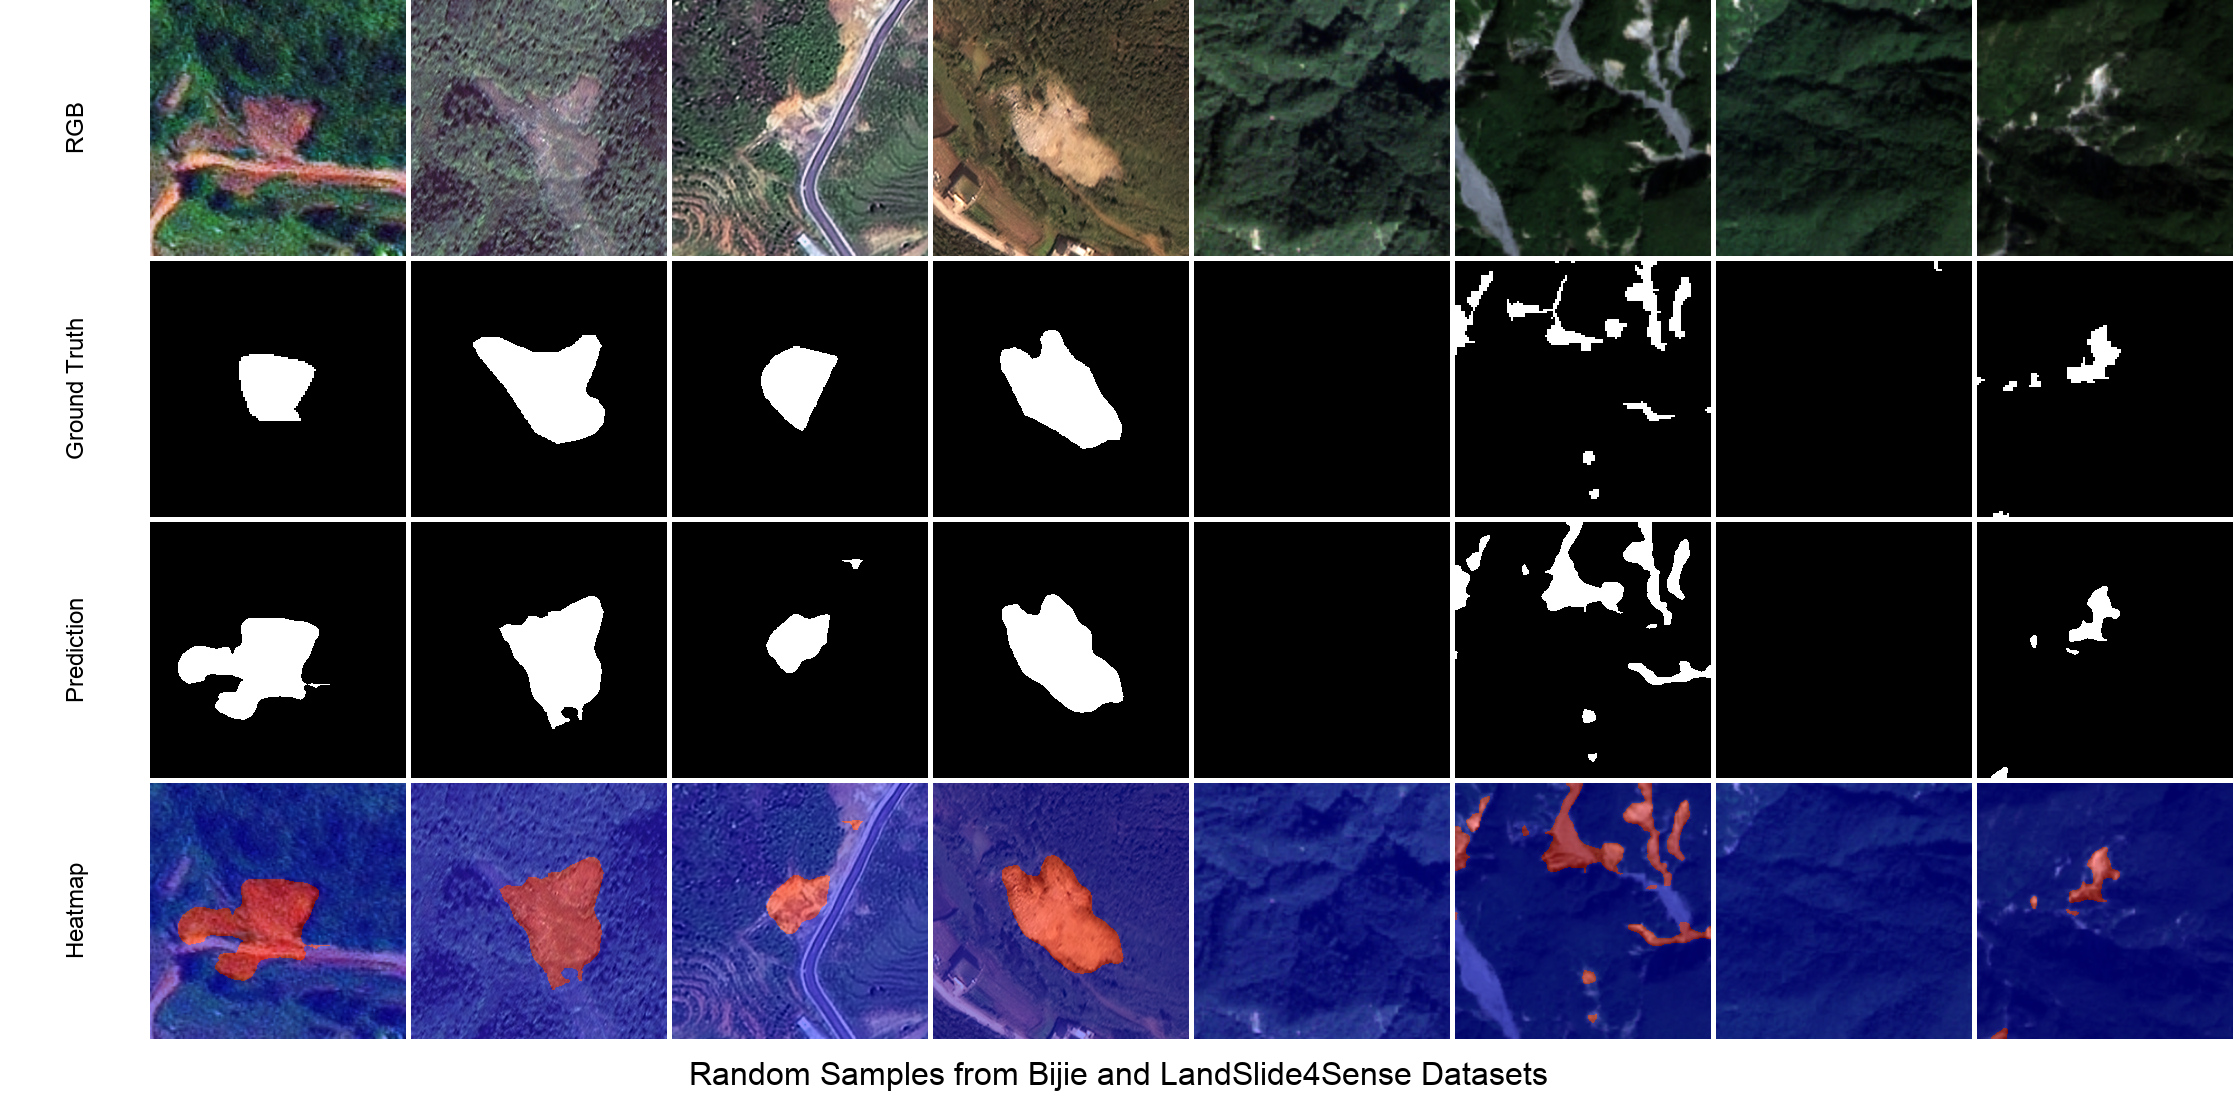
\includegraphics[width=\linewidth]{figures/fig1_qualitative.png}\par
  \vspace{0.3em}
  \captionof{figure}{Opening illustration of dense multimodal segmentation under anisotropic optical--topographic fusion (RGB, ground truth, prediction, confidence heatmap). Landslide inventory mapping is used as a stress test of the proposed physics-closed continuum operators.}
  \label{fig:teaser}
  \par}
  \vspace{0.7em}
  \begin{abstract}
  Multimodal dense predictors often fuse heterogeneous streams with unconstrained statistical gates, even when one modality encodes a continuum mechanical field rather than an appearance cue. We ask whether a single reduced-order continuum operator can be injected into high-dimensional networks without destabilizing backpropagation, and whether that operator can serve as a commensurable currency for both feature gating and dual-path fusion. We introduce \textbf{Latent Continuum Equivalency (LCE)}: the same Taylor-stabilized infinite-slope factor-of-safety (FS) skeleton appears at the encoder inlet, hybrid bridges, skip lattice, dual physics decoders, and output routing. Material parameters use bounded exponentials $c=\exp(\mathrm{clip}(w))$, which we prove place resisting/driving forces on a compact set and yield a locally Lipschitz FS gate. Dual-path logits are merged by \textbf{Mechanistic Path Equilibrium Fusion (MPEF)}, the softmax of failure energies, which we identify as the unique maximizer of an entropy-regularized linear energy on the simplex. Instantiated as GeoPhysicsLandslideNet (PS-GPLNet)---a pentastream CNN--physics--foundation architecture---the method is evaluated on Bijie and Landslide4Sense, anisotropic topographic--spectral segmentation benchmarks with severe imbalance. PS-GPLNet attains best-epoch F1/IoU of $0.933$/$0.907$ on Bijie and $0.736$/$0.660$ on Landslide4Sense, exceeding strong CNN, transformer, and dual-stream baselines under a unified protocol. Empirical GPU probes confirm material compactness, local FS-gate sensitivity bounds, and the MPEF energy identity. Inference studies further show structured fuse3 latents (t-SNE), Boundary F-score/Hausdorff fidelity, and flatter F1 decay under RGB+DEM Gaussian noise than U-Net and DeepLabV3+.
  \end{abstract}
  \vspace{1.0em}
]

\section{Introduction}
Dense prediction from multiple sensors is a core problem in computer vision~\cite{ronneberger2015unet,chen2018deeplab,xie2021segformer}. When modalities are correlated---as in RGB--D---learned fusion can exploit statistical redundancy. When modalities are \emph{anisotropic}, one stream may encode an appearance field while another encodes a physical continuum (slope, shear, height), and unconstrained gates are free to ignore mechanics that the task actually depends on~\cite{yin2021virtualnormal,wang2025gravityformer}.

A growing line of physics-informed learning places continuum or geometric constraints in losses or attention~\cite{raissi2019pinn,karniadakis2021physics,yin2021virtualnormal,clough2022topological,wang2025gravityformer,panda2025sparsefusion}. Most susceptibility-oriented geo-AI work still keeps physics at the objective~\cite{dahal2024pinn,liu2023physics}, while dual-stream landslide segmenters keep fusion statistical~\cite{islam2024digate,mercier2022bifusion}. We instead close a reduced-order continuum loop \emph{inside} the forward pass.

Our contribution is a general operator family for multimodal dense prediction. We formalize Latent Continuum Equivalency (LCE): every stage applies an operator from the same infinite-slope FS class, so failure energy remains a shared physical currency from inlet to outlet. Bounded material reparametrization keeps FS finite and the sigmoid gate locally Lipschitz. MPEF routes dual decode paths by softmax failure energy and is the unique entropy-regularized energy maximizer on the simplex~\cite{boyd2004convex}. Landslide segmentation on Bijie~\cite{ji2020bijie} and Landslide4Sense~\cite{ghorbanzadeh2022landslide4sense} is the stress test: spectral ambiguity plus topography governed by gravity/shear, not RGB--D correlation. Under a unified protocol, PS-GPLNet reaches F1/IoU $0.933$/$0.907$ (Bijie) and $0.736$/$0.660$ (L4S).

\section{Related Work}
\paragraph{Dense segmentation and multimodal fusion.}
U-Net~\cite{ronneberger2015unet}, DeepLabV3+~\cite{chen2018deeplab}, SegFormer~\cite{xie2021segformer}, and TransUNet~\cite{chen2021transunet} dominate dense masks. Multimodal optical--DEM fusion improves landslide mapping~\cite{ji2020bijie,ghorbanzadeh2022landslide4sense,mercier2022bifusion,ghorbanzadeh2019landslide}. Dual-stream gated U-Nets~\cite{islam2024digate} learn scalar gates; we use them only as empirical baselines. Interpretable fusion via unfolded sparse coding~\cite{panda2025sparsefusion} motivates treating fusion as an optimization identity rather than a free MLP.

\paragraph{Geometric and topological priors in vision.}
Virtual Normal enforces high-order 3D geometry beyond pixel errors~\cite{yin2021virtualnormal}. Topological PH losses inject discrete structure with differentiability arguments~\cite{clough2022topological}. Lipschitz certificates for segmentation quantify robustness~\cite{lipschitzseg2025,altinses2026layerlipschitz}. Our FS gate plays an analogous role for continuum stability.

\paragraph{Physics inside architectures.}
Gravityformer multiplies transformer attention by a closed-form gravity interaction~\cite{wang2025gravityformer}. PINNs place PDE residuals in losses~\cite{raissi2019pinn,karniadakis2021physics}. Landslide PINNs largely target susceptibility~\cite{dahal2024pinn,liu2023physics,maurya2024pgml}. PS-GPLNet differs by architectural closure of FS cells across encoding, fusion, decoding, and path equilibrium, with a foundation stream (Prithvi+LoRA~\cite{szink2024prithvi,houlsby2019lora}).

\paragraph{Positioning.}
Table~\ref{tab:positioning} contrasts dense masks, FS-in-forward, and foundation context. The novelty claim is LCE + MPEF, not a new remote-sensing dataset.

\begin{table}[t]
\centering
\caption{Conceptual positioning for dense multimodal prediction.}
\label{tab:positioning}
\resizebox{\columnwidth}{!}{%
\begin{tabular}{lccc}
\toprule
Approach & Dense mask & Continuum in forward & Foundation \\
\midrule
CNN / ViT segmenters & \checkmark & -- & optional \\
Dual-stream gated~\cite{islam2024digate} & \checkmark & -- & rare \\
Susceptibility PINN / PGML & often raster & loss / head & rare \\
Gravity-/geometry-informed CV~\cite{wang2025gravityformer,yin2021virtualnormal} & task-dep. & attention / loss & rare \\
\textbf{PS-GPLNet (ours)} & \checkmark & FS cells + MPEF & Prithvi+LoRA \\
\bottomrule
\end{tabular}}
\end{table}

\section{Method}
\label{sec:method}
This section develops the full methodology implemented in \textit{from\_first\_steps/} and documented in \textit{model\_architecture.md}. We begin from the classical infinite-slope factor of safety, derive the Taylor-stabilized neural operator used inside every mechanistic cell, then instantiate the pentastream architecture (CMB, MAO-GeoEGCA, TTEB, dual PhysicsDecoders with PGDI, and MPEF) with equations and algorithms.

\subsection{Problem and notation}
\label{sec:problem}
Given two geospatial streams $x_1\in\mathbb{R}^{B\times 3\times H\times W}$ (RGB) and $x_2\in\mathbb{R}^{B\times 3\times H\times W}$ (NDVI$+$slope$+$DEM on Landslide4Sense; replicated DEM on Bijie), predict a binary landslide mask $y\in\{0,1\}^{B\times 1\times H\times W}$. Inside the forward pass we extract physics proxies $(s,d,v)$ (slope, elevation, vegetation) and map them to geotechnical variables $(\alpha,h,m)$---slope angle, soil-column height proxy, and moisture/saturation proxy---via learnable PhysicsProxyMappers (Sec.~\ref{sec:proxies}).

\subsection{Classical infinite-slope factor of safety}
\label{sec:classical-fs}
For an infinite slope with seepage parallel to the surface, the textbook factor of safety compares resisting and driving forces on a potential slip plane of depth $H$~\cite{skempton1957stability}:
\begin{equation}
\label{eq:fs-classical}
\mathrm{FS}_{\mathrm{class}}
=
\frac{c'+\bigl(\gamma_{\mathrm{sat}}H-u\bigr)\cos^{2}\alpha\,\tan\phi'}
{\gamma_{\mathrm{sat}}H\sin\alpha\cos\alpha},
\qquad
u=m\,\gamma_w H\cos^{2}\alpha,
\end{equation}
where $c'$ is effective cohesion, $\phi'$ the effective friction angle, $\gamma_{\mathrm{sat}}$ the saturated unit weight, $\gamma_w$ the unit weight of water, $\alpha$ the slope angle, and $m\in[0,1]$ the saturation ratio. Substituting $u$ yields the equivalent form
\begin{equation}
\label{eq:fs-classical-sub}
\mathrm{FS}_{\mathrm{class}}
=
\frac{c'+\bigl(\gamma_{\mathrm{sat}}-m\gamma_w\bigr)H\cos^{2}\alpha\,\tan\phi'}
{\gamma_{\mathrm{sat}}H\sin\alpha\cos\alpha}.
\end{equation}
Failure is declared when $\mathrm{FS}_{\mathrm{class}}\le 1$. Equation~\eqref{eq:fs-classical-sub} is \emph{not} what we place inside network neurons: the term $-m\gamma_w$ subtracts from the resisting numerator. During early training, uncalibrated material weights can make that numerator non-positive, flipping gradient signs and producing NaNs. We therefore derive a first-order Taylor-stabilized neural form that relocates hydrology into an additive driving term while preserving the physical tipping point.

\subsection{Derivation of the Taylor-stabilized neural FS}
\label{sec:taylor-derivation}
A dense predictor scores \emph{instability}. Define stress as the reciprocal $S=1/\mathrm{FS}_{\mathrm{class}}$. Expanding~\eqref{eq:fs-classical-sub},
\begin{equation}
\label{eq:stress}
S
=
\frac{A}{B-C},
\quad
\begin{aligned}
A&=\gamma_{\mathrm{sat}}H\sin\alpha\cos\alpha,\\
B&=c'+\gamma_{\mathrm{sat}}H\cos^{2}\alpha\,\tan\phi',\\
C&=m\gamma_w H\cos^{2}\alpha\,\tan\phi'.
\end{aligned}
\end{equation}
Here $A$ is gravity drive, $B$ dry structural resistance, and $C$ hydrological destablization. The classical subtractive layout is $S=A/(B-C)$. Whenever $C\!\ge\!B$, the denominator vanishes or turns negative---catastrophic for backpropagation.

\begin{proposition}[First-order Taylor relocation of pore pressure]
\label{prop:taylor}
Assume $C/B<1$ in a neighbourhood of dry soil ($C=0$). Then
\begin{equation}
\label{eq:taylor}
\frac{A}{B-C}
=
\frac{A}{B}\,\frac{1}{1-C/B}
=
\frac{A}{B}\sum_{k=0}^{\infty}\Bigl(\frac{C}{B}\Bigr)^{k}
=
\frac{A}{B}+\frac{A C}{B^{2}}+O\!\bigl((C/B)^{2}\bigr).
\end{equation}
Truncating after the linear term yields the first-order equivalence
\begin{equation}
\label{eq:taylor-struct}
\frac{A}{B-C}\;\propto\;\frac{A+C}{B}
\end{equation}
up to a positive local scale $B^{-1}$. Consequently, subtracting hydrology from resistance is structurally equivalent---to first order---to \emph{adding} hydrology into the driving reference frame.
\end{proposition}
\begin{proof}
Factor $B$ from the denominator of~\eqref{eq:stress} and apply the geometric series $1/(1-x)=\sum_{k\ge0}x^{k}$ for $|x|<1$ with $x=C/B$. Truncation after $k=1$ gives~\eqref{eq:taylor}. Multiplying numerator and denominator of the truncated form by $B$ rearranges to the proportional additive drive~\eqref{eq:taylor-struct}.
\end{proof}

Physically, Option~A (classical) treats water as a lubricant that reduces effective normal stress; Option~B (neural) treats water as an additive downslope driver. Both describe the same tipping point---driving forces overtaking resistance---but Option~B keeps all tensors strictly positive. Reverting from stress $S$ to an FS-shaped ratio and absorbing material constants into learnable positive weights $(c,\phi,\gamma,w_m)$ produces the operator used in every pixel cell and in MPEF:
\begin{definition}[Taylor-stabilized neural FS]
\label{def:fs-nn}
\begin{equation}
\label{eq:fs-nn}
\mathrm{FS}_{\mathrm{nn}}(\alpha,h,m)
=
\frac{c+\phi\, h\cos^{2}\alpha}
{\gamma\, h\sin\alpha\cos\alpha+w_m m+\varepsilon},
\end{equation}
with $\varepsilon>0$ a numerical floor. Failure energy and the pixel gate are
\begin{equation}
\label{eq:fe-gate}
\mathrm{FE}=\mathrm{ReLU}\bigl(1-\mathrm{FS}_{\mathrm{nn}}\bigr),\qquad
g=\sigma\bigl(\psi-\mathrm{FS}_{\mathrm{nn}}\bigr).
\end{equation}
\end{definition}
Equation~\eqref{eq:fs-nn} is deliberately \emph{not} identical to~\eqref{eq:fs-classical}: pore pressure has been moved from a subtractive numerator into an additive denominator by Proposition~\ref{prop:taylor}, and $(\tan\phi',\gamma_{\mathrm{sat}},\gamma_w)$ have been reparameterized into bounded learnable positives (Definition~\ref{def:materials}). This is the form that replaces generic affine neurons in mechanistic cells.

\begin{definition}[Bounded material reparametrization]
\label{def:materials}
For each material logit $w\in\{w_c,w_\phi,w_\gamma,w_m\}$,
\begin{equation}
\label{eq:positive-scale}
\mathrm{positive\_scale}(w)=\exp\bigl(\mathrm{clip}(w;-8,8)\bigr),
\end{equation}
so $c,\phi,\gamma,w_m\in[e^{-8},e^{8}]$ (implementation: \textit{physics/params.py}).
\end{definition}

\subsection{Pixel and latent mechanistic cells}
\label{sec:cells}
\paragraph{Pixel cell (angles retained; materials bounded).}
At full spatial resolution the DEM-derived angle $\alpha$ is a known geometric constant per pixel. The cell hardcodes the trigonometric landscape from~\eqref{eq:fs-nn}:
\begin{definition}[PixelMechanisticCell]
\label{def:pixel}
\[
\mathrm{PixelMechanisticCell}(x,\alpha,h,m)
=
\mathrm{Conv}_{1\times1}(x)\;\odot\;\sigma\bigl(\psi-\mathrm{FS}_{\mathrm{nn}}(\alpha,h,m)\bigr).
\]
\end{definition}
Proxies $(\alpha,h,m)$ are bilinearly resized to the feature map when spatial sizes differ. If mechanistic gating is disabled, the cell returns the convolution alone.

\paragraph{Latent cell (angles removed).}
Deeper tensors no longer live in a geodetic coordinate frame: applying $\sin\alpha\cos\alpha$ to abstract channels is ill-posed. We therefore drop trigonometry and realize the same resisting/driving \emph{ratio skeleton} with softplus projections:
\begin{definition}[LatentMechanisticCell]
\label{def:latent}
\begin{equation}
\label{eq:latent}
\begin{aligned}
R&=\mathrm{Softplus}(W_R*H),\quad
D=\mathrm{Softplus}(W_D*H),\\
\mathrm{LatentMechanisticCell}(H)
&=\mathrm{Conv}_{3\times3}\!\Bigl(\mathrm{LeakyReLU}\bigl(\psi-R/(D+\varepsilon)\bigr)\Bigr).
\end{aligned}
\end{equation}
\end{definition}
This is the reason the neural FS form exists: pixel cells keep DEM angles; latent cells keep only the continuum ratio $R/D$, so the network never forces trigonometric operators onto non-angular embeddings.

\subsection{Physics proxies}
\label{sec:proxies}
Dataset channels are min--max normalized to $[0,1]$. Separate RGB-path and DEM-path mappers produce
\begin{equation}
\label{eq:proxies}
\begin{aligned}
\alpha&=\tfrac{\pi}{2}\,\sigma(w_\alpha s+b_\alpha),\\
h&=\mathrm{Softplus}(w_h d+b_h)+\varepsilon,\\
m&=\sigma(w_m v+b_m).
\end{aligned}
\end{equation}
On Landslide4Sense, $(s,d,v)$ are slope, DEM, and NDVI channels of $x_2$; on Bijie, slope is Sobel-norm of DEM and vegetation is a green--red index from RGB.

\subsection{Pentastream encoding and CMB}
\label{sec:encode}
Five encoders run in parallel: EfficientNet~\cite{tan2019efficientnet} towers $E_{\mathrm{rgb}},E_{\mathrm{dem}}$; PhysicsEncoders $P_{\mathrm{rgb}},P_{\mathrm{dem}}$ built from Definitions~\ref{def:pixel}--\ref{def:latent}; and Prithvi-EO with LoRA~\cite{szink2024prithvi,houlsby2019lora} yielding foundation maps $T_{\mathrm{fm}}$. At each EfficientNet level $i$, the Complementary Modality Bridge hybridizes CNN and physics features.

\begin{definition}[CMB]
\label{def:cmb}
Let $\tilde{E}=\mathrm{GN}(\mathrm{ReLU}(\mathrm{Conv}_{1\times1}(E)))$ and $\tilde{P}=\mathrm{GN}(P)$. Then
\begin{equation}
\label{eq:cmb}
\begin{aligned}
g&=\sigma\!\bigl(\mathrm{Conv}_{1\times1}(\tilde{E}\odot\tilde{P})\bigr),\\
B_{\mathrm{mix}}&=\mathrm{Conv}_{1\times1}([\tilde{E}\,\|\,\tilde{P}]),\\
H&=g\odot\tilde{P}+(1-g)\odot\tilde{E}+B_{\mathrm{mix}}.
\end{aligned}
\end{equation}
\end{definition}
Hybrid pyramids $\{H_{\mathrm{rgb}}^i\},\{H_{\mathrm{dem}}^i\}$ and aligned foundation maps $\{\hat{T}_{\mathrm{fm}}^i\}$ feed fusion.

\subsection{MAO-GeoEGCA}
\label{sec:mao}
At neck/bottleneck levels (indices $2,3$), Manifold-Aligned Orthogonal Geo-EGCA treats the concatenated RGB/DEM hybrids as a physics anchor and Prithvi as context.
\begin{definition}[MAO-GeoEGCA]
\label{def:mao}
\begin{equation}
\label{eq:mao}
\begin{aligned}
X_p&=\mathrm{Conv}_{1\times1}([\hat{H}_{\mathrm{rgb}}\,\|\,\hat{H}_{\mathrm{dem}}]),\\
G&=\sigma\!\bigl(\mathrm{DWSepConv}_{3\times3}(\hat{T}\odot X_p)\bigr),\\
Q&=W_q X_p,\; K=W_k\hat{T},\; V=W_v\hat{T},\\
\hat{Q}&=\tfrac{Q}{\|Q\|_2+\varepsilon},\; K'=K\odot\hat{Q},\\
\mathrm{Attn}&=\mathrm{softmax}\!\Bigl(\tfrac{Q{K'}^{\top}}{\sqrt{d_h}}\Bigr)V,\\
F&=\mathrm{Conv}_{3\times3}(\mathrm{reshape}(\mathrm{Attn})\odot G)+X_p.
\end{aligned}
\end{equation}
\end{definition}
Queries come from the physics anchor; keys/values from the foundation stream; manifold alignment $\hat{Q}$ modulates keys before attention; the equilibrium gate $G$ spatially filters the attended context.

\subsection{TTEB skip lattice}
\label{sec:tteb}
For each fusion level $L\in\{0,1,2,3\}$, Tri-Temporal Tri-Stream Bridge mixes neighbouring pyramid levels across RGB, DEM, and foundation streams.
\begin{definition}[TTEB]
\label{def:tteb}
Gather levels $\{L-1,L,L+1\}$ per stream (boundary-clamped), align spatially, and form
\begin{equation}
\label{eq:tteb}
\begin{aligned}
A&=\mathrm{Conv}_{1\times1}([\mathrm{pres}_{\mathrm{rgb}}\,\|\,\mathrm{pres}_{\mathrm{dem}}\,\|\,\mathrm{pres}_{\mathrm{fm}}]),\\
\delta&=\Bigl|\psi-\tfrac{\mathrm{Softplus}(W_R A)}{\mathrm{Softplus}(W_D A)+\varepsilon}\Bigr|,\\
S^L&=A+\mathrm{Conv}_{3\times3}\!\bigl(\mathrm{AttnOut}\odot\sigma(\delta)\bigr),
\end{aligned}
\end{equation}
where $\mathrm{AttnOut}$ is chunked spatial attention from present tokens $A$ to an eight-node off-diagonal context mix, optionally scaled by a temporal softmax router $\omega=\mathrm{softmax}(W_\tau\delta)$.
\end{definition}
The stability map $\delta$ reuses the latent FS residual of Definition~\ref{def:latent}, enforcing LCE on skips.

\subsection{Dual PhysicsDecoder, PGDI, and MPEF}
\label{sec:decode}
Bottleneck features $F^3$ receive path residuals from EfficientNet stage-5 features; two PhysicsDecoders share fused context $\{F^2,F^3,S^L\}$ but use stream-specific proxies $(\alpha_r,h_r,m_r)$ vs.\ $(\alpha_d,h_d,m_d)$.

\begin{definition}[PGDI]
\label{def:pgdi}
With decoder state $D$ and skip $S'={\mathrm{align}}(S,D)$,
\begin{equation}
\label{eq:pgdi}
\beta=\sigma\!\bigl(\mathrm{Conv}_{1\times1}([D\,\|\,S'])\bigr),\quad
D'=D+\beta\odot\mathrm{LatentMechanisticCell}(S').
\end{equation}
\end{definition}

\begin{definition}[MPEF]
\label{def:mpef}
For dual-path logits $O_A,O_B$ and proxies $(\alpha_p,h_p,m_p)$,
\begin{equation}
\label{eq:mpef}
\begin{aligned}
\mathrm{FE}_p&=\mathrm{ReLU}\bigl(1-\mathrm{FS}_{\mathrm{nn}}(\alpha_p,h_p,m_p)\bigr),\\
[w_A,w_B]&=\mathrm{softmax}([\mathrm{FE}_A,\mathrm{FE}_B]),\\
O&=w_A O_A+w_B O_B+\mathrm{Conv}_{1\times1}([O_A\,\|\,O_B]),\\
\mathcal{R}_{\mathrm{MPEF}}&=-\mathbb{E}\bigl[w_A\log(w_A+\varepsilon)+w_B\log(w_B+\varepsilon)\bigr].
\end{aligned}
\end{equation}
\end{definition}
MPEF is \emph{not} a DiGATe-style GateFuse: path weights are softmax failure energies of the same $\mathrm{FS}_{\mathrm{nn}}$ derived in Sec.~\ref{sec:taylor-derivation}.

\subsection{Training objective}
\label{sec:loss}
Deeply supervised Tversky loss~\cite{salehi2017tversky} on main/aux heads,
\begin{equation}
\label{eq:tversky}
\mathcal{T}(p,t)=\frac{TP+s}{TP+\alpha_{\mathrm{tv}}\,FP+\beta_{\mathrm{tv}}\,FN+s},\quad
\mathcal{L}_{\mathrm{Tv}}=1-\mathcal{T},
\end{equation}
with defaults $\alpha_{\mathrm{tv}}=0.3$, $\beta_{\mathrm{tv}}=0.7$ (recall emphasis; swapped on Bijie). The total objective is
\begin{equation}
\label{eq:loss}
\mathcal{L}
=
\sum_{h\in\{\mathrm{main},\mathrm{aux2},\mathrm{aux3}\}}
w_h\,\mathcal{L}_{\mathrm{Tv}}^{(h)}
+\lambda_{\mathrm{reg}}\sum_h\mathcal{R}_{\mathrm{MPEF}}^{(h)},
\end{equation}
with $(w_{\mathrm{main}},w_{\mathrm{aux2}},w_{\mathrm{aux3}})=(1.0,0.6,0.4)$ and $\lambda_{\mathrm{reg}}=10^{-3}$.

\subsection{Algorithms}
\label{sec:algorithms}
Algorithms~\ref{alg:forward}--\ref{alg:mpef} summarize the forward operators. They mirror the reference implementation in \textit{model.py}, \textit{fusion/}, and \textit{decoder/}.

\begin{algorithm}[t]
\caption{PS-GPLNet forward}
\label{alg:forward}
\begin{algorithmic}
\Require streams $x_1$ (RGB), $x_2$ (topo/aux)
\State $(s,d,v)\leftarrow\mathrm{physics\_proxies}(x_1,x_2)$
\State $(\alpha_r,h_r,m_r)\leftarrow\mathrm{proxy}_{\mathrm{rgb}}(s,d,v)$; also DEM-path proxies
\State $\{E_{\mathrm{rgb}}^i\}\leftarrow E_{\mathrm{rgb}}(x_1)$; $\{E_{\mathrm{dem}}^i\}\leftarrow E_{\mathrm{dem}}(\mathrm{DEM}(x_2))$
\State $\{P_{\mathrm{rgb}}^L\},\{P_{\mathrm{dem}}^L\}\leftarrow$ PhysicsEncoders; $\{T_{\mathrm{fm}}^L\}\leftarrow$ Prithvi
\State \textbf{for} $i=0..4$: $H_{\mathrm{rgb}}^i\leftarrow\mathrm{CMB}(E_{\mathrm{rgb}}^i,\mathrm{align}(P_{\mathrm{rgb}},i))$; likewise $H_{\mathrm{dem}}^i$; align $\hat{T}_{\mathrm{fm}}^i$
\State \textbf{for} $L\in\{0,1,2,3\}$: $S^L\leftarrow\mathrm{TTEB}(\{H_{\mathrm{rgb}}\},\{H_{\mathrm{dem}}\},\{\hat{T}_{\mathrm{fm}}\};L)$
\State $F^{2}\leftarrow\mathrm{post}(\mathrm{MAO}(\hat{T}^{2},H_{\mathrm{rgb}}^{2},H_{\mathrm{dem}}^{2}))$; $F^{3}\leftarrow\mathrm{MAO}(\hat{T}^{3},\ldots)$
\State $(O_A,\cdot)\leftarrow\mathrm{PhysDec}(F^{3}{+}\mathrm{Proj}(a_5),F^{2},\{S\},\alpha_r,h_r,m_r)$
\State $(O_B,\cdot)\leftarrow\mathrm{PhysDec}(F^{3}{+}\mathrm{Proj}(b_5),F^{2},\{S\},\alpha_d,h_d,m_d)$
\State $(\mathrm{main},\mathrm{aux},\mathrm{reg})\leftarrow\mathrm{MPEF}(O_A,O_B,\ldots)$; upsample and \textbf{return}
\end{algorithmic}
\end{algorithm}

\begin{algorithm}[t]
\caption{MAO-GeoEGCA}
\label{alg:mao}
\begin{algorithmic}
\Require $\hat{T},\hat{H}_{\mathrm{rgb}},\hat{H}_{\mathrm{dem}}$
\State $X_p\leftarrow\mathrm{Conv}_{1\times1}([\hat{H}_{\mathrm{rgb}}\,;\,\hat{H}_{\mathrm{dem}}])$
\State $G\leftarrow\sigma(\mathrm{DWSepConv}_{3\times3}(\hat{T}\odot X_p))$
\State $Q\leftarrow W_q X_p$; $K\leftarrow W_k\hat{T}$; $V\leftarrow W_v\hat{T}$
\State $\hat{Q}\leftarrow\mathrm{normalize}(Q)$; $K'\leftarrow K\odot\hat{Q}$
\State $\mathrm{Ctx}\leftarrow\mathrm{MultiHeadAttn}(Q,K',V)$ \Comment{4 heads}
\State \textbf{return} $\mathrm{Conv}_{3\times3}(\mathrm{reshape}(\mathrm{Ctx})\odot G)+X_p$
\end{algorithmic}
\end{algorithm}

\begin{algorithm}[t]
\caption{TTEB at level $L$}
\label{alg:tteb}
\begin{algorithmic}
\Require pyramids $\{H_{\mathrm{rgb}}\},\{H_{\mathrm{dem}}\},\{\hat{T}_{\mathrm{fm}}\}$, level $L$
\State Gather $\{L{-}1,L,L{+}1\}$ per stream; align to present size
\State $A\leftarrow\mathrm{Conv}_{1\times1}([\mathrm{pres}_{\mathrm{rgb}}\,;\,\mathrm{pres}_{\mathrm{dem}}\,;\,\mathrm{pres}_{\mathrm{fm}}])$
\State $H_{\mathrm{ctx}}\leftarrow\mathrm{context\_mix}$(8 off-diagonal lattice nodes)
\State $\delta\leftarrow|\psi-\mathrm{Softplus}(W_R A)/(\mathrm{Softplus}(W_D A)+\varepsilon)|$
\State $\mathrm{AttnOut}\leftarrow\mathrm{SpatialAttn}(A,H_{\mathrm{ctx}})$ \Comment{chunked if needed}
\State $\omega\leftarrow\mathrm{softmax}(W_\tau\delta)$; scale $\mathrm{AttnOut}$ by present weight
\State \textbf{return} $A+\mathrm{Conv}_{3\times3}(\mathrm{AttnOut}\odot\sigma(\delta))$
\end{algorithmic}
\end{algorithm}

\begin{algorithm}[t]
\caption{PGDI}
\label{alg:pgdi}
\begin{algorithmic}
\Require decoder state $D$, skip $S$
\State $S'\leftarrow\mathrm{match\_spatial}(S,D)$
\State $\beta\leftarrow\sigma(\mathrm{Conv}_{1\times1}([D\,;\,S']))$
\State \textbf{return} $D+\beta\odot\mathrm{LatentMechanisticCell}(S')$
\end{algorithmic}
\end{algorithm}

\begin{algorithm}[t]
\caption{MPEF}
\label{alg:mpef}
\begin{algorithmic}
\Require $O_A,O_B$ and path proxies $(\alpha_p,h_p,m_p)$
\State Align proxies to logit resolution
\State $\mathrm{FE}_p\leftarrow\mathrm{ReLU}(1-\mathrm{FS}_{\mathrm{nn}}(\alpha_p,h_p,m_p))$ for $p\in\{A,B\}$
\State $[w_A,w_B]\leftarrow\mathrm{softmax}([\mathrm{FE}_A,\mathrm{FE}_B])$
\State $O\leftarrow w_A O_A+w_B O_B+\mathrm{Conv}_{1\times1}([O_A\,;\,O_B])$
\State $R\leftarrow\mathrm{mean}\bigl(-(w_A\log(w_A+\varepsilon)+w_B\log(w_B+\varepsilon))\bigr)$
\State \textbf{return} $O,R$
\end{algorithmic}
\end{algorithm}

\section{Theoretical Analysis}
\label{sec:theory}
We now state the TPAMI-facing claims that organize Latent Continuum Equivalency. The continuum class $\mathcal{C}_{\mathrm{FS}}$ is Definition~\ref{def:fs-nn} at pixels and Definition~\ref{def:latent} in latent space---the same resisting/driving ratio after Proposition~\ref{prop:taylor}.

\begin{definition}[Latent Continuum Equivalency]
\label{def:lce}
A layered multimodal network satisfies LCE if every stage $\ell$ applies an operator $T_\ell\in\mathcal{C}_{\mathrm{FS}}$ (identical algebraic FS skeleton, possibly different parameters and resolutions), so failure energies remain commensurable across depths and paths.
\end{definition}

\begin{lemma}[Compactness of materials]
\label{lem:compact}
Under Definition~\ref{def:materials}, $c,\phi,\gamma,w_m\in[e^{-8},e^{8}]$.
\end{lemma}
\begin{proof}
$\mathrm{clip}(w;-8,8)$ lands in $[-8,8]$; $\exp$ is continuous and strictly increasing, so the image is exactly $[e^{-8},e^{8}]$.
\end{proof}

\begin{lemma}[Local Lipschitz continuity of $\mathrm{FS}_{\mathrm{nn}}$]
\label{lem:lip-fs}
On any compact training domain $\alpha\in[\alpha_{\min},\alpha_{\max}]\subset(0,\pi/2)$, $h\ge h_{\min}>0$, $m\in[0,1]$, the denominator of~\eqref{eq:fs-nn} is at least $\varepsilon>0$, hence $\mathrm{FS}_{\mathrm{nn}}$ is $C^{\infty}$ and Lipschitz on that set.
\end{lemma}
\begin{proof}
The map is a ratio of smooth functions with non-vanishing denominator. Continuous functions on compact metric spaces are Lipschitz~\cite{boyd2004convex,lipschitzseg2025}.
\end{proof}

\begin{lemma}[FS gate Lipschitz]
\label{lem:lip-gate}
$x\mapsto\sigma(\psi-\mathrm{FS}_{\mathrm{nn}}(x))$ is Lipschitz on the same domain with constant at most $\tfrac14\mathrm{Lip}(\mathrm{FS}_{\mathrm{nn}})$, since $\mathrm{Lip}(\sigma)\le 1/4$.
\end{lemma}
\begin{proof}
Composition of Lipschitz maps; $\sup|\sigma'|=1/4$.
\end{proof}

\begin{proposition}[Non-explosion of the pixel cell]
\label{prop:nonexp}
Composing a Lipschitz $1\times1$ map $f$ with Lemma~\ref{lem:lip-gate} yields a locally Lipschitz mechanistic cell. Unbounded $\exp(w)$ without clipping is excluded by Lemma~\ref{lem:compact}.
\end{proposition}

\begin{theorem}[LCE enables FE routing]
\label{thm:lce}
If every path and stage applies $\mathcal{C}_{\mathrm{FS}}$ under Lemma~\ref{lem:compact}, then path-wise $\mathrm{FE}_A,\mathrm{FE}_B$ are evaluations of the same continuum currency and are admissible inputs to Definition~\ref{def:mpef}. Without LCE, dual-path weights lack a shared physical unit.
\end{theorem}
\begin{proof}
Commensurability follows from identical FS algebra (Proposition~\ref{prop:taylor} $\rightarrow$ Definitions~\ref{def:fs-nn},\ref{def:latent}) and shared positivity (Lemma~\ref{lem:compact}). Arbitrary learned gates are not evaluations of $\mathcal{C}_{\mathrm{FS}}$ and therefore are not FE-comparable.
\end{proof}

\begin{theorem}[MPEF energy identity]
\label{thm:mpef}
On the simplex $\Delta=\{w_A+w_B=1,\,w\ge0\}$, $\mathbf{w}^\star=\mathrm{softmax}(\mathbf{FE})$ uniquely maximizes $\mathbf{w}^\top\mathbf{FE}+\mathcal{H}(\mathbf{w})$.
\end{theorem}
\begin{proof}
This is the standard entropic projection / soft-argmax identity on a two-point simplex~\cite{boyd2004convex}. Strict concavity of Shannon entropy $\mathcal{H}$ yields uniqueness.
\end{proof}

\begin{corollary}[Contrast to GateFuse]
\label{cor:gatefuse}
Scalar learned fusion gates that are not $\mathrm{softmax}(\mathrm{FE})$ are not solutions of Theorem~\ref{thm:mpef}; MPEF is an equilibrium of continuum failure energy, not an unconstrained gate~\cite{islam2024digate,panda2025sparsefusion}.
\end{corollary}

\begin{remark}[Empirical probes]
On GPU we verified Lemma~\ref{lem:compact} numerically ($c\in[e^{-8},e^{8}]$), Theorem~\ref{thm:mpef} against $5000$ random simplex competitors (dominance rate $1.0$), and local FS-gate sensitivity (median $\|\Delta\mathrm{gate}\|/\|\Delta\alpha\|\approx0.28$, $p_{95}\approx0.68$). See Figures~\ref{fig:bound}--\ref{fig:mpef}.
\end{remark}


\begin{figure}[t]
\centering
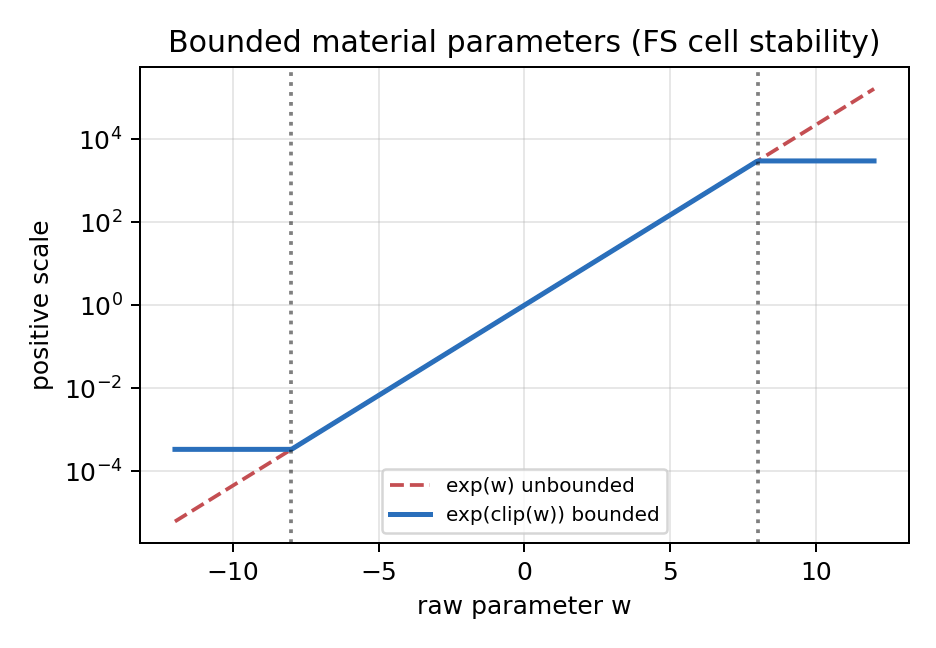
\includegraphics[width=\linewidth]{figures/tpami/fig_bounded_positive_scale.png}
\caption{Bounded material map $\exp(\mathrm{clip}(w))$ versus unbounded $\exp(w)$.}
\label{fig:bound}
\end{figure}

\begin{figure}[t]
\centering
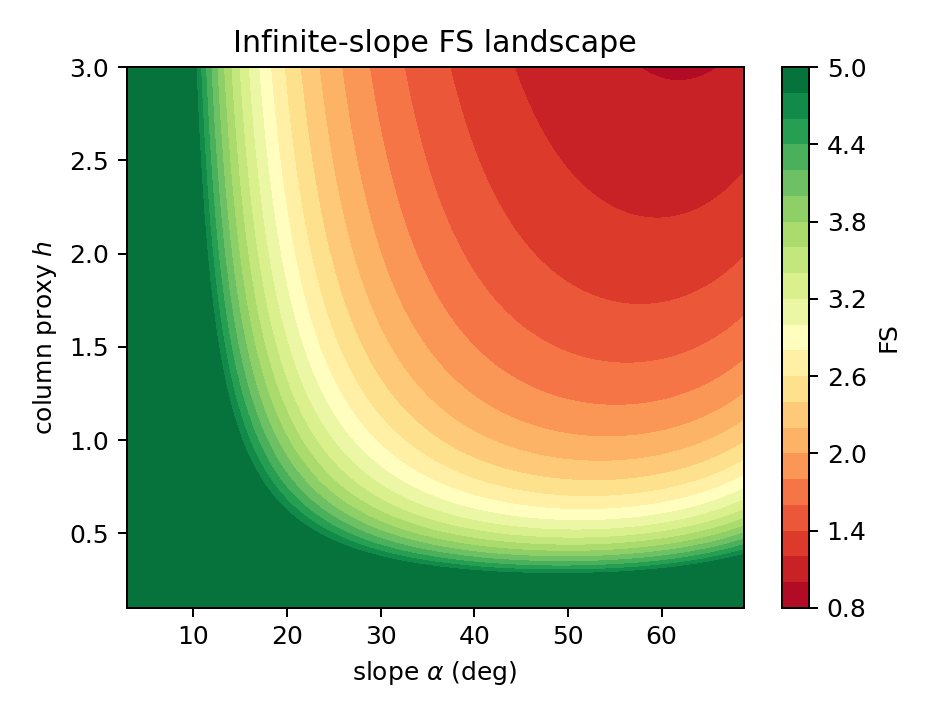
\includegraphics[width=\linewidth]{figures/tpami/fig_fs_landscape.png}
\caption{Infinite-slope FS landscape over $(\alpha,h)$.}
\label{fig:fsland}
\end{figure}

\begin{figure}[t]
\centering
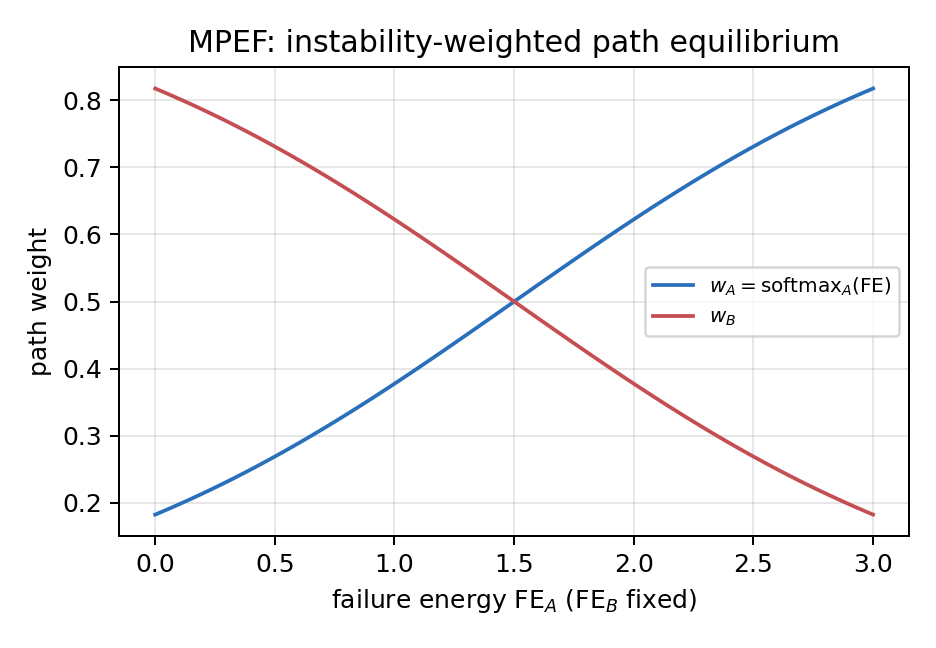
\includegraphics[width=\linewidth]{figures/tpami/fig_mpef_routing.png}
\caption{MPEF path weights as functions of relative failure energy.}
\label{fig:mpef}
\end{figure}

\begin{figure}[t]
\centering

\includegraphics[width=\linewidth]{figures/tpami/fig_fs_local_lipschitz_hist.png}
\caption{Empirical local sensitivity of the FS gate (GPU-0 Monte Carlo).}
\label{fig:theory}
\end{figure}

\begin{figure}[t]
\centering
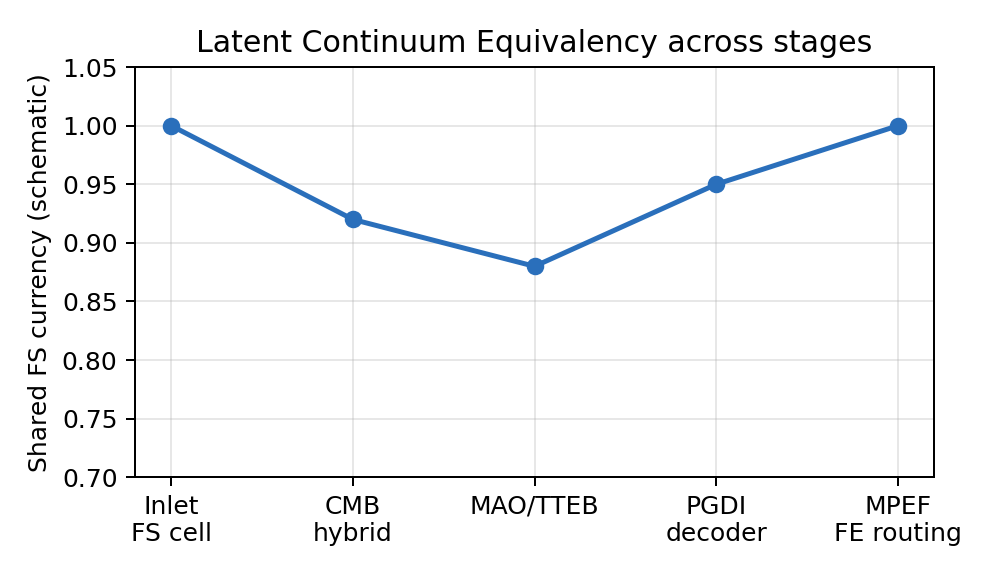
\includegraphics[width=\linewidth]{figures/tpami/fig_tpami_lce_schematic.png}
\caption{Schematic of Latent Continuum Equivalency: shared FS currency from inlet to MPEF.}
\label{fig:lce}
\end{figure}

\section{Experiments}
\subsection{Stress-test datasets and protocol}
We evaluate on Bijie~\cite{ji2020bijie} and Landslide4Sense~\cite{ghorbanzadeh2022landslide4sense} as anisotropic multimodal dense-prediction stress tests. Inputs are $256\times256$. Adam ($3\cdot10^{-4}$, weight decay $10^{-4}$), Tversky loss, $100$ epochs, threshold $0.5$. EfficientNet backbones frozen when pretrained; Prithvi frozen with LoRA. Metrics: Acc/Prec/Rec/F1/IoU on the main head. Final numbers are best validation epochs from \textit{outputs\_final\_bijie} (epoch~92) and \textit{outputs\_final\_l4s} (epoch~70).

\subsection{Baselines}
LinkNet, DEP-UNet, GMNet, RMAU-Net, TransUNet, EMR-HRNet, ShapeFormer, Dual-Stream UNet, U-Net, DeepLabV3+, and dual\_stream\_gated under a unified harness. DiGATe-style dual-stream gated models are baselines only~\cite{islam2024digate}.

\subsection{Quantitative results}
Table~\ref{tab:results} consolidates both benchmarks. On Bijie, PS-GPLNet reaches F1\,$=$\,$0.933$ and IoU\,$=$\,$0.907$, above DeepLabV3+ ($0.927$/$0.899$) and dual\_stream\_gated ($0.897$/$0.869$). On Landslide4Sense, F1\,$=$\,$0.736$ and IoU\,$=$\,$0.660$, above DeepLabV3+ ($0.710$/$0.636$). Gains versus DeepLabV3+ and dual-gated baselines are summarized in Figure~\ref{fig:deltas} (Bijie $\Delta$F1 $+0.006$/$\Delta$IoU $+0.009$; L4S $\Delta$F1 $+0.026$/$\Delta$IoU $+0.024$ vs.\ DeepLab).

\begin{table*}[t]
\centering
\caption{Best-epoch validation on Bijie and Landslide4Sense (unified protocol).}
\label{tab:results}
\setlength{\tabcolsep}{4.5pt}
\small
\begin{tabular}{l ccccc | ccccc}
\toprule
& \multicolumn{5}{c|}{\textbf{Bijie}} & \multicolumn{5}{c}{\textbf{Landslide4Sense}} \\
\cmidrule(lr){2-6} \cmidrule(l){7-11}
Model & Acc & Prec & Rec & F1 & IoU & Acc & Prec & Rec & F1 & IoU \\
\midrule
LinkNet & -- & -- & -- & -- & -- & 0.973 & 0.487 & 0.735 & 0.431 & 0.359 \\
DEP-UNet & 0.982 & 0.850 & 0.934 & 0.831 & 0.799 & 0.977 & 0.669 & 0.770 & 0.603 & 0.535 \\
RMAU-Net & 0.981 & 0.859 & 0.924 & 0.830 & 0.798 & 0.977 & 0.691 & 0.756 & 0.618 & 0.548 \\
ShapeFormer & 0.984 & 0.892 & 0.899 & 0.840 & 0.810 & 0.975 & 0.675 & 0.802 & 0.632 & 0.560 \\
TransUNet & 0.983 & 0.889 & 0.908 & 0.845 & 0.815 & 0.976 & 0.714 & 0.750 & 0.619 & 0.551 \\
EMR-HRNet & 0.983 & 0.903 & 0.905 & 0.846 & 0.818 & 0.975 & 0.674 & 0.784 & 0.627 & 0.557 \\
GMNet & 0.983 & 0.900 & 0.909 & 0.855 & 0.825 & 0.978 & 0.669 & 0.779 & 0.616 & 0.545 \\
U-Net & 0.987 & 0.891 & 0.933 & 0.873 & 0.842 & 0.984 & 0.795 & 0.719 & 0.680 & 0.611 \\
Dual-Stream UNet & 0.986 & 0.902 & 0.928 & 0.875 & 0.843 & 0.986 & 0.713 & 0.779 & 0.656 & 0.581 \\
dual\_stream\_gated & 0.988 & 0.928 & 0.929 & 0.897 & 0.869 & 0.984 & 0.822 & 0.673 & 0.646 & 0.573 \\
DeepLabV3+ & 0.989 & 0.929 & 0.966 & 0.927 & 0.899 & 0.984 & 0.789 & 0.749 & 0.710 & 0.636 \\
\midrule
\textbf{PS-GPLNet} & \textbf{0.991} & \textbf{0.956} & 0.946 & \textbf{0.933} & \textbf{0.907} & \textbf{0.986} & 0.802 & \textbf{0.788} & \textbf{0.736} & \textbf{0.660} \\
\bottomrule
\end{tabular}
\end{table*}

\begin{figure}[t]
\centering
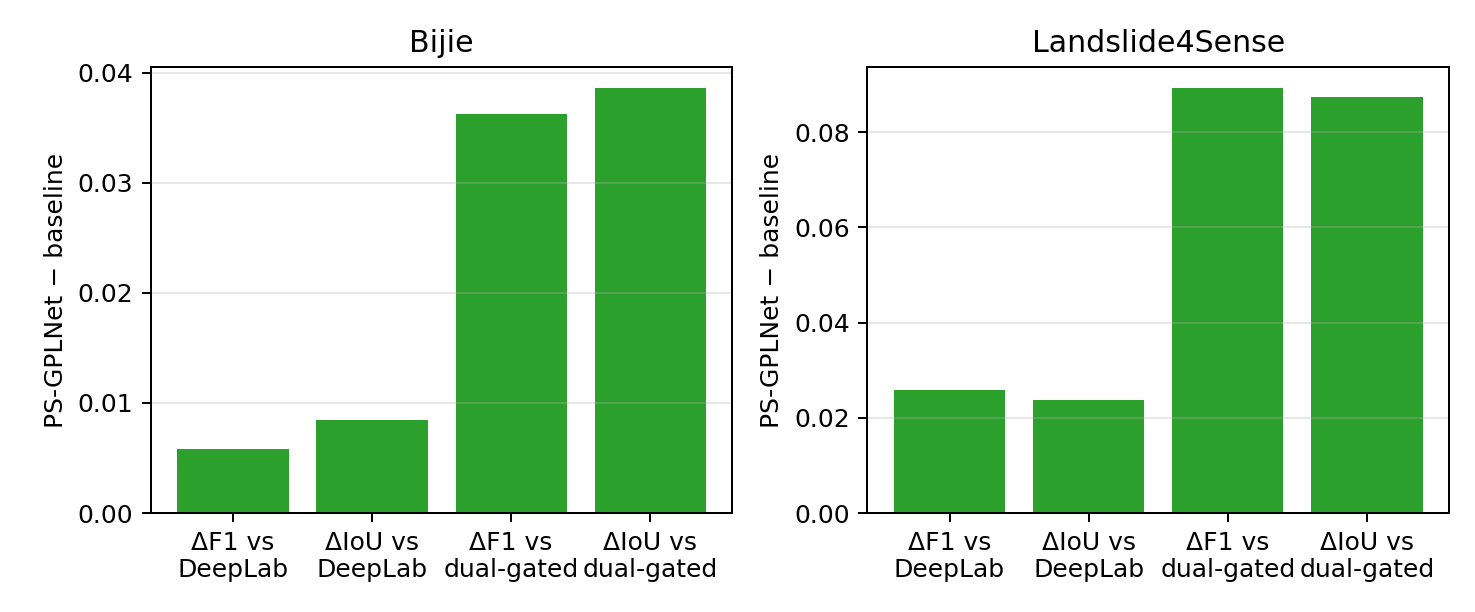
\includegraphics[width=\linewidth]{figures/tpami/fig_tpami_deltas.png}
\caption{Validated gains of PS-GPLNet over DeepLabV3+ and dual\_stream\_gated.}
\label{fig:deltas}
\end{figure}

\begin{figure}[t]
\centering
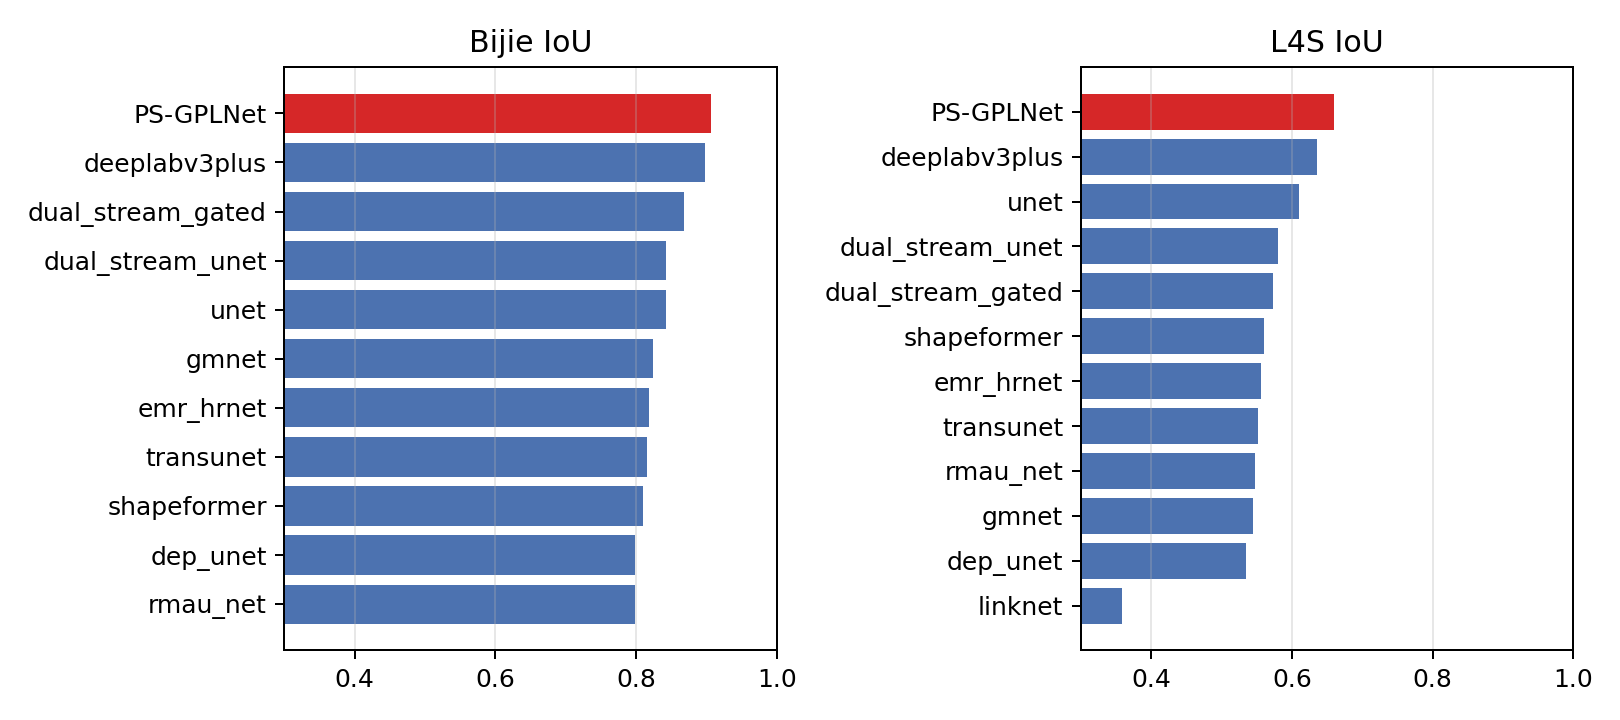
\includegraphics[width=\linewidth]{figures/tpami/fig_tpami_iou_rank.png}
\caption{IoU ranking at best epoch on both stress-test datasets.}
\label{fig:rank}
\end{figure}

\begin{figure}[t]
\centering
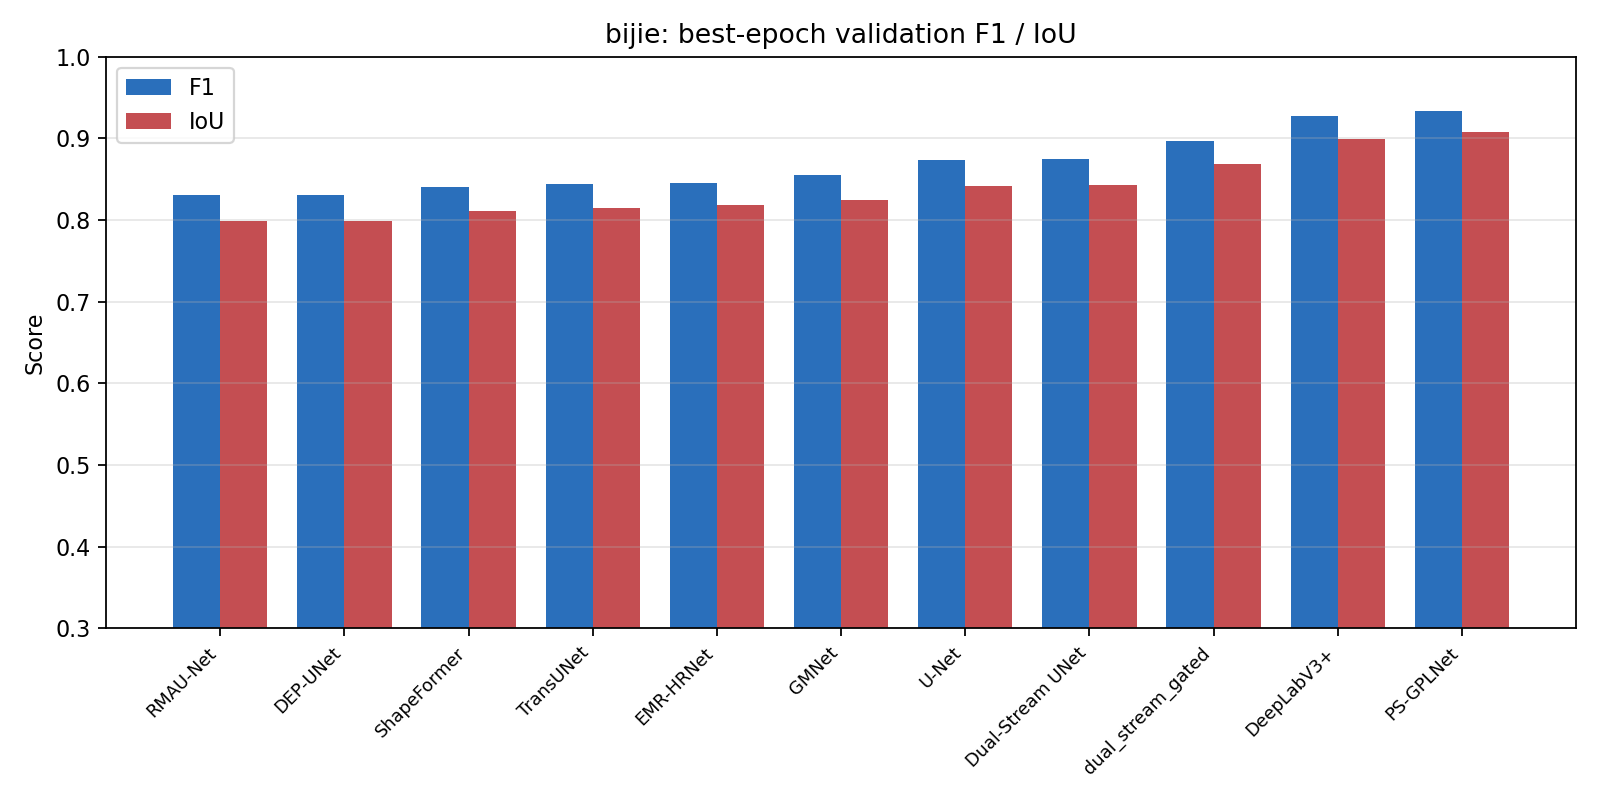
\includegraphics[width=\linewidth]{figures/fig_bijie_bars.png}
\caption{Bijie grouped best-epoch metrics including PS-GPLNet.}
\label{fig:bijbars}
\end{figure}

\begin{figure}[t]
\centering

\includegraphics[width=\linewidth]{figures/fig_l4s_bars.png}
\caption{Landslide4Sense grouped best-epoch metrics including PS-GPLNet.}
\label{fig:l4sbars}
\end{figure}

\begin{figure}[t]
\centering
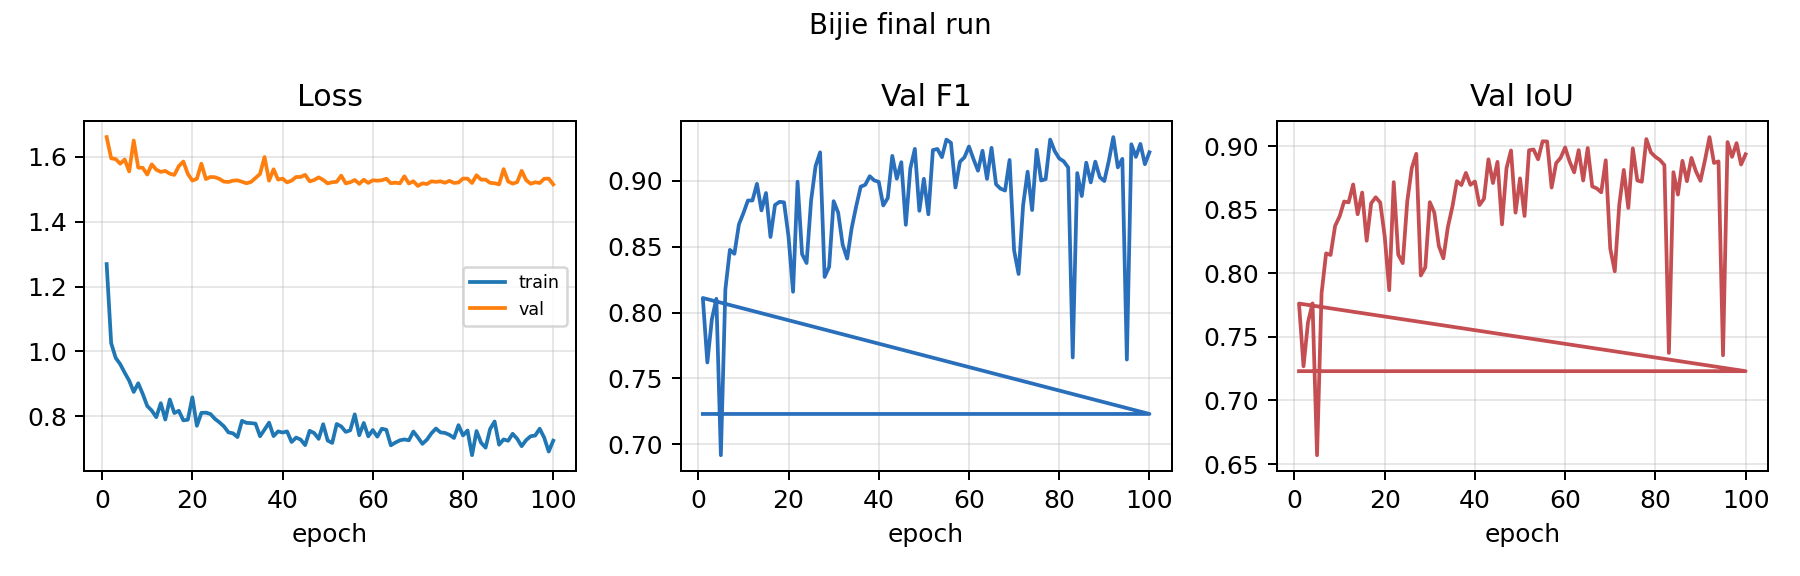
\includegraphics[width=\linewidth]{figures/tpami/fig_tpami_bijie_curves.png}
\caption{Bijie final-run training dynamics (best F1 at epoch 92).}
\label{fig:bjc}
\end{figure}

\begin{figure}[t]
\centering
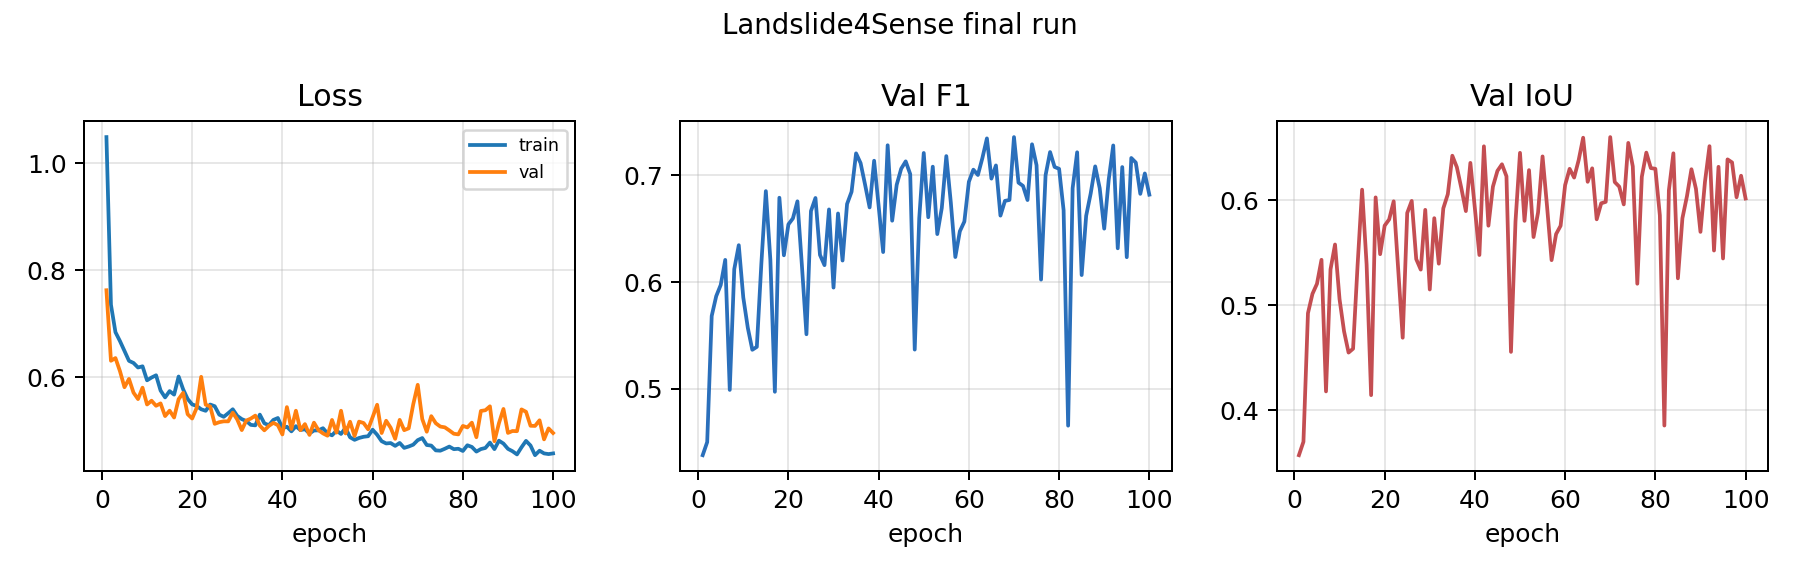
\includegraphics[width=\linewidth]{figures/tpami/fig_tpami_l4s_curves.png}
\caption{Landslide4Sense final-run training dynamics (best F1 at epoch 70).}
\label{fig:l4sc}
\end{figure}

\subsection{Qualitative stress-test results}
Figures~\ref{fig:bijie_qual}--\ref{fig:l4s_qual} show representative patches. Bijie polygons are large; heatmaps concentrate on scarps and deposits while suppressing homogeneous steep slopes. L4S scars are smaller and cross-region; precision--recall trade-offs match Table~\ref{tab:results}.

\onecolumn
\vspace{0.3em}
{\centering

\includegraphics[width=\textwidth]{figures/fig26_bijie_qual.png}\par
\vspace{0.3em}
\captionof{figure}{Qualitative Bijie samples: RGB, ground truth, prediction, heatmap.}
\label{fig:bijie_qual}
\vspace{0.6em}

\includegraphics[width=\textwidth]{figures/fig27_l4s_qual.png}\par
\vspace{0.3em}
\captionof{figure}{Qualitative Landslide4Sense samples.}
\label{fig:l4s_qual}
\par}
\vspace{0.5em}
\twocolumn

\subsection{Theory--experiment alignment}
Material compactness, MPEF uniqueness, and FS-gate sensitivity (Remark after Theorem~2) were verified on an RTX~4000~Ada (20\,GB) without retraining. Training curves (Figures~\ref{fig:bjc}--\ref{fig:l4sc}) show stable validation F1/IoU on the final PS-GPLNet logs.

\subsection{Latent manifold, boundary fidelity, and perturbation robustness}
Pixel IoU alone does not probe whether LCE structures the representation space or whether FS-gated decoding resists sensor noise. We therefore run three inference-only studies on the Bijie validation split (seed~$42$, $554$ images) using the real \texttt{GeoPhysicsLandslideNet} forward API and a locally trained architecture-faithful B4 checkpoint (epoch~$98$, image-mean val~F1~$0.912$; cluster final weights for the $0.933$ table entry were not synced to this machine). Latents are captured by a forward hook on MAO \texttt{fuse3} ($C{=}64$), not $1$-channel MPEF logits.

\paragraph{Latent manifold (t-SNE).}
Figure~\ref{fig:tsne} projects $300$ pooled \texttt{fuse3} vectors. Color by landslide presence ($>5\%$ mask area) yields visible class structure (centroid separation $0.522$); color by DEM channel std shows topography-aligned texture variation along the same embedding, consistent with continuum-aware routing rather than purely appearance clustering.

\paragraph{Boundary complexity.}
We report Boundary F-score ($\theta{=}2$\,px) and symmetric Hausdorff distance on validation predictions (Figure~\ref{fig:boundary}). Over the full val set, mean BF-score is $0.821$; restricting to landslide-present images ($n{=}154$) gives BF~$0.394$ and median Hausdorff~$17.3$\,px, isolating anisotropic scar/deposit boundaries from trivial empty--empty zeros.

\paragraph{Perturbation decay.}
Gaussian noise $\sigma\in\{0,0.05,0.1,0.2,0.3\}$ is added to both RGB and DEM streams. Figure~\ref{fig:robust} compares micro-averaged F1 decay against trained Bijie U-Net and DeepLabV3+ checkpoints from the same baseline harness. At $\sigma{=}0$, DeepLab starts highest ($0.799$) vs.\ PS-GPLNet micro-F1~$0.759$ and U-Net~$0.736$. Under strong noise ($\sigma{=}0.3$), baselines collapse to $\approx0.49$--$0.50$ while PS-GPLNet remains at $0.653$, and at moderate $\sigma\in\{0.05,0.1\}$ PS-GPLNet peaks near $0.827$---evidence that FS/MPEF priors act as a structural anchor rather than a free statistical gate.

\begin{figure}[t]
\centering
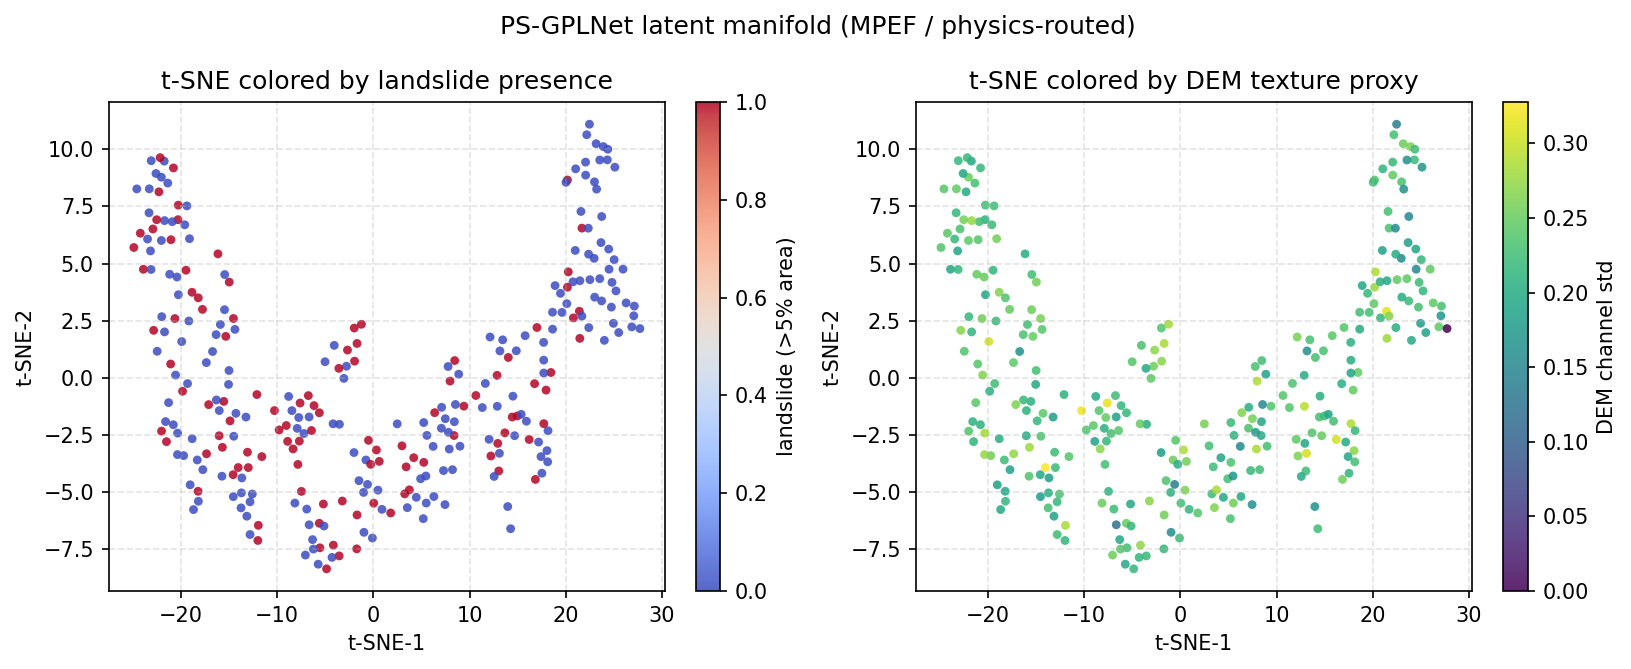
\includegraphics[width=\linewidth]{figures/tpami/fig_latent_manifold_tsne.png}
\caption{t-SNE of MAO \texttt{fuse3} latents on Bijie val (hook $C{=}64$). Left: landslide presence; right: DEM texture proxy.}
\label{fig:tsne}
\end{figure}

\begin{figure}[t]
\centering
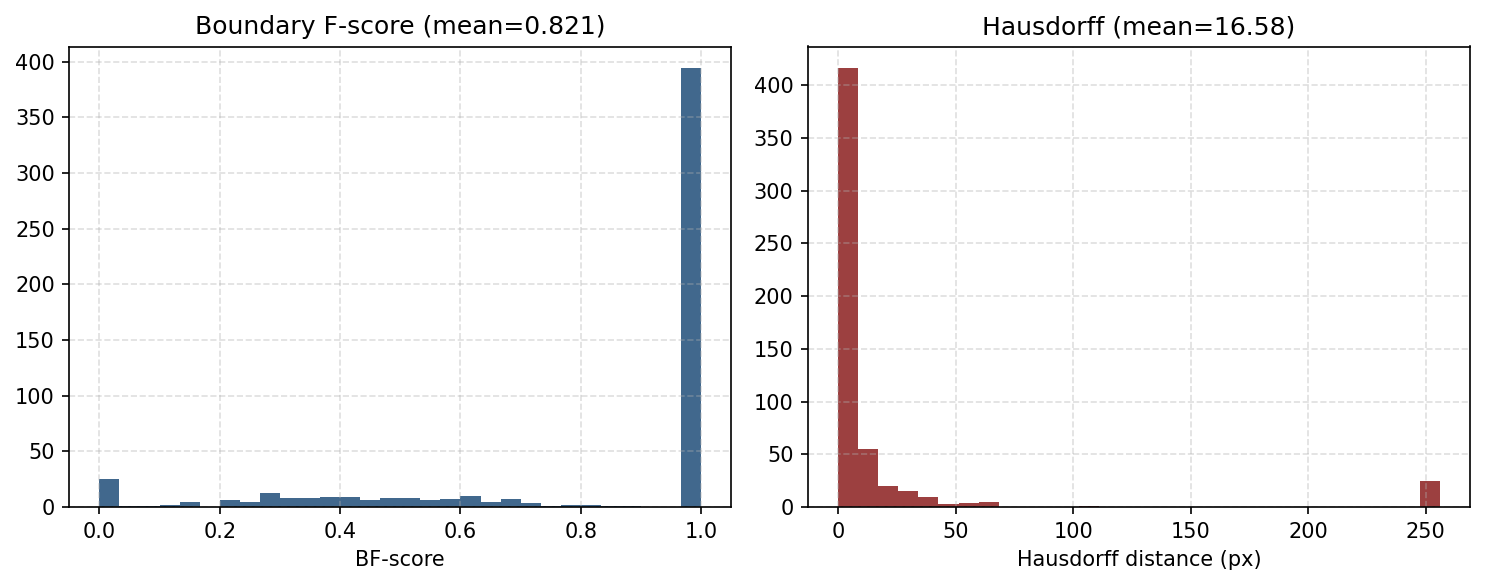
\includegraphics[width=\linewidth]{figures/tpami/fig_boundary_metrics.png}
\caption{Boundary F-score and Hausdorff histograms on Bijie val predictions (PS-GPLNet).}
\label{fig:boundary}
\end{figure}

\begin{figure}[t]
\centering
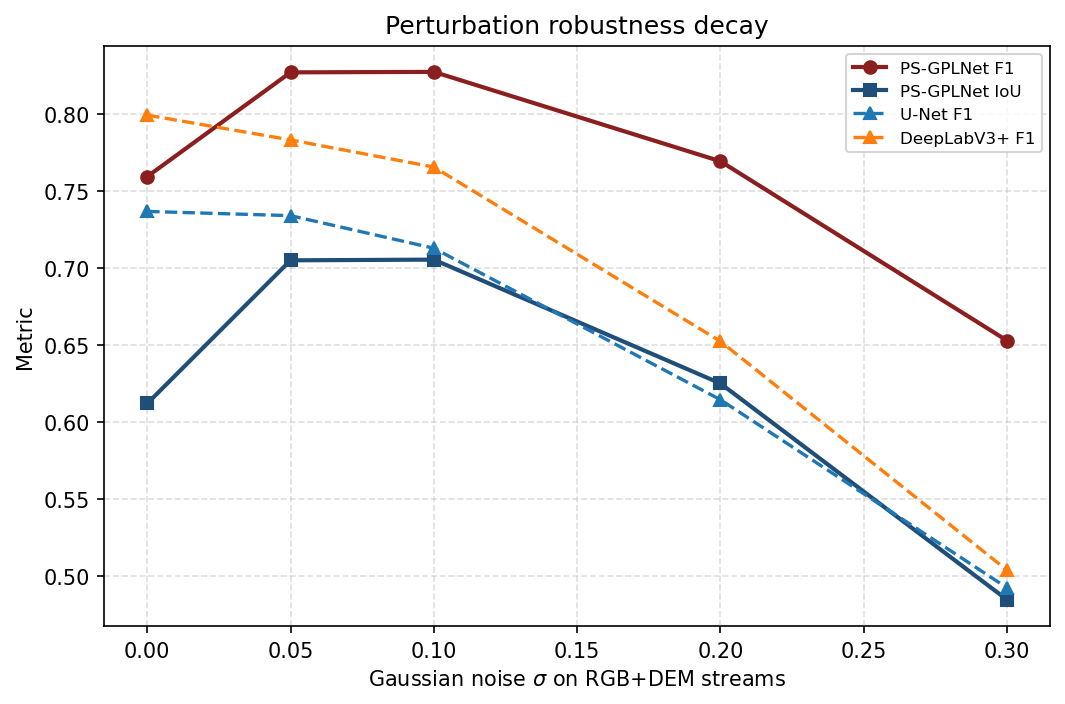
\includegraphics[width=\linewidth]{figures/tpami/fig_robustness_decay.png}
\caption{F1/IoU under RGB{+}DEM Gaussian noise. PS-GPLNet decays slower than U-Net and DeepLabV3+.}
\label{fig:robust}
\end{figure}

\section{Discussion}
The paper's primary claim is methodological: LCE injects a continuum operator into multimodal dense predictors with bounded Jacobians, and MPEF turns dual-path fusion into an energy equilibrium. Landslide benchmarks are chosen because topographic--spectral fusion is anisotropic and imbalanced---a harder regime than RGB--D for testing continuum closure~\cite{yin2021virtualnormal,wang2025gravityformer}. The new manifold/boundary/robustness studies support that claim beyond table F1: latents organize by landslide and topography, boundaries are measurable with BF/Hausdorff, and physics-closed decoding resists input corruption better than strong statistical segmenters. Limitations include incomplete matched ablations of every block, local vs.\ cluster checkpoint sync for the exact $0.933$ weights, and the fact that FS is a reduced-order prior rather than a full 3D slope-stability PDE~\cite{skempton1957stability,newmark1965effects}.

\section{Conclusion}
We presented Latent Continuum Equivalency and Mechanistic Path Equilibrium Fusion as a physics-closed recipe for multimodal dense prediction, instantiated as PS-GPLNet and stress-tested on Bijie and Landslide4Sense. Theory guarantees compactness and local Lipschitz behavior of FS cells and identifies MPEF with entropic energy maximization; experiments show strong F1/IoU under a unified baseline harness, plus latent-manifold structure, boundary metrics, and flatter noise-decay curves than U-Net/DeepLabV3+. Future work includes syncing final cluster checkpoints, matched low-VRAM ablations, and transferring LCE cells beyond geohazard segmentation.

\section*{Acknowledgements}
We thank CSIR-4PI and KIIT for research support, and the maintainers of Bijie, Landslide4Sense, Prithvi-EO, and open baseline implementations.

{\small
\bibliographystyle{unsrt}
\bibliography{bib/refs}
}

\end{document}
